\chapter{Environement et jeu}

\section{Représentation du monde}
    \subsection{Géométrie du monde}
        La premiere chose à faire était de définir des constantes, stuctures et variables qui allait nous servir tout au long du projet tel que : \\
        
        \noindent Les directions :
        \begin{center}
            \begin{multicols}{2}
                NORTH \\ NEAST \\ NWEST \\ WEST \\ SOUTH \\ SWEST \\ SWEST \\ EAST
            \end{multicols}
        \end{center}
        
        \noindent Le type de couleur de la case :
        \begin{center}
            NO-COLOR \hspace{1cm} WHITE \hspace{1cm} BLACK \\
        \end{center}
        \noindent L'occupant de la case :
        \begin{center}
            NO-SORT \hspace{2cm} SIMPLE-PAWN \\ 
        \end{center}
        
        \noindent Cette catégorie est voué à s'agrandir au vu de l'ajout de différentes sorte de pions par la suite. \\
        
        \noindent Nous avons également eu besoin des constantes pour définir le monde : \\
        

        \begin{itemize}
            \item Taille: WORLD-SIZE,
            \item Longueur: WIDTH,
            \item Largeur: HEIGHT,
            \item Nombre de maximum de cases: UNIT-MAX,
            \item Nombre de joueurs: NB-PLAYERS,
        \end{itemize}
        
        \noindent \\ Avec ces variables, nous avons créés la structure "world" qui nous à permis d'assigner à chaque case du monde une couleur et un état d'occupation, ce qui vas grandement nous servire dans la suite du projet.
        
    \subsection{Plateau de jeu}
        Il faut definir un plateau de jeu pour l'utilisateur. Nous avons decidé de faire celui-ci de forme torique afin rendre le jeu plus modulable. Il a donc fallut nous affranchire des effets de bord à l'aide de modulos. Ce choix a aussi été fait pour des raisons d'antissipation des futures modifications, qui seront plus faciles a implémenter en partant d'un modèle très généraliste tel que le tore (Figure \textbf{\ref{fig:tore_de_jeu}}).\\
        \newline
            \begin{figure}[H]
                \centering
                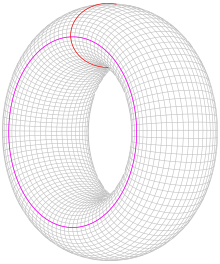
\includegraphics[scale=0.4]{tor.png}
                \caption{tore de jeu}
                \label{fig:tore_de_jeu}
            \end{figure}
  
        Par défault, nous avons implémentés des relations entre cases de type hexagonal (Figure \textbf{\ref{fig:pavage_hexagonal}}), comme il nous l'était imposé en début de projet. Cependant, dans le cadre d'un achievement nous avons également implémenté des changement de terrains, qui impactent les relations faisant passer notre monde d'un pavage hexagonal, à un pavage carré (Figure \textbf{\ref{fig:pavage_carre}}) ou triagulaire (Figure \textbf{\ref{fig:pavage_triangulaire}}). Ces changements interviennent au bout d'un certain nombre de tour, nombre qui peut être paramétré par le joueur.
        
        \begin{figure}[H]
            \centering
            \begin{subfigure}{0.3\textwidth}
                \centering
                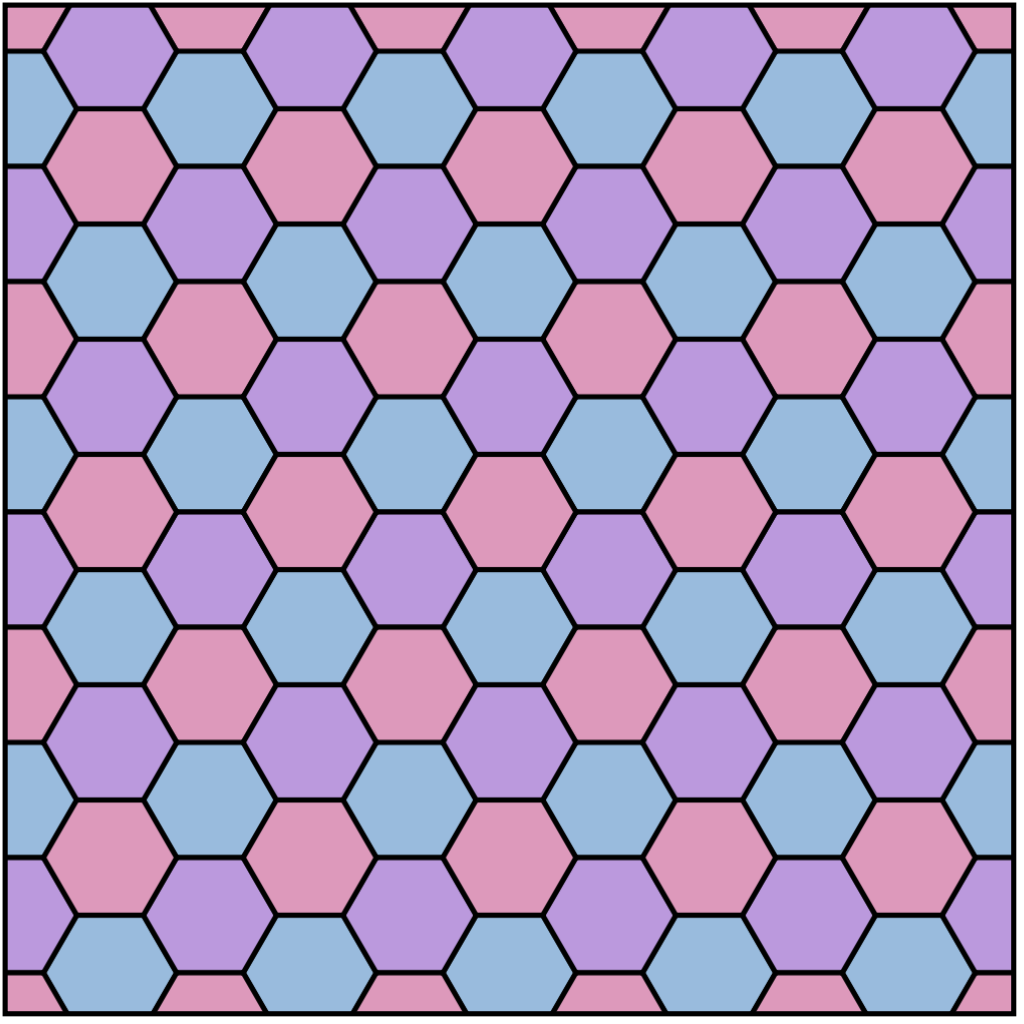
\includegraphics[width=\textwidth]{pavage_hexagonal.png}
                \caption{Pavage hexagonal}
                \label{fig:pavage_hexagonal}
            \end{subfigure}
            \quad
            \begin{subfigure}{0.3\textwidth}
                \centering
                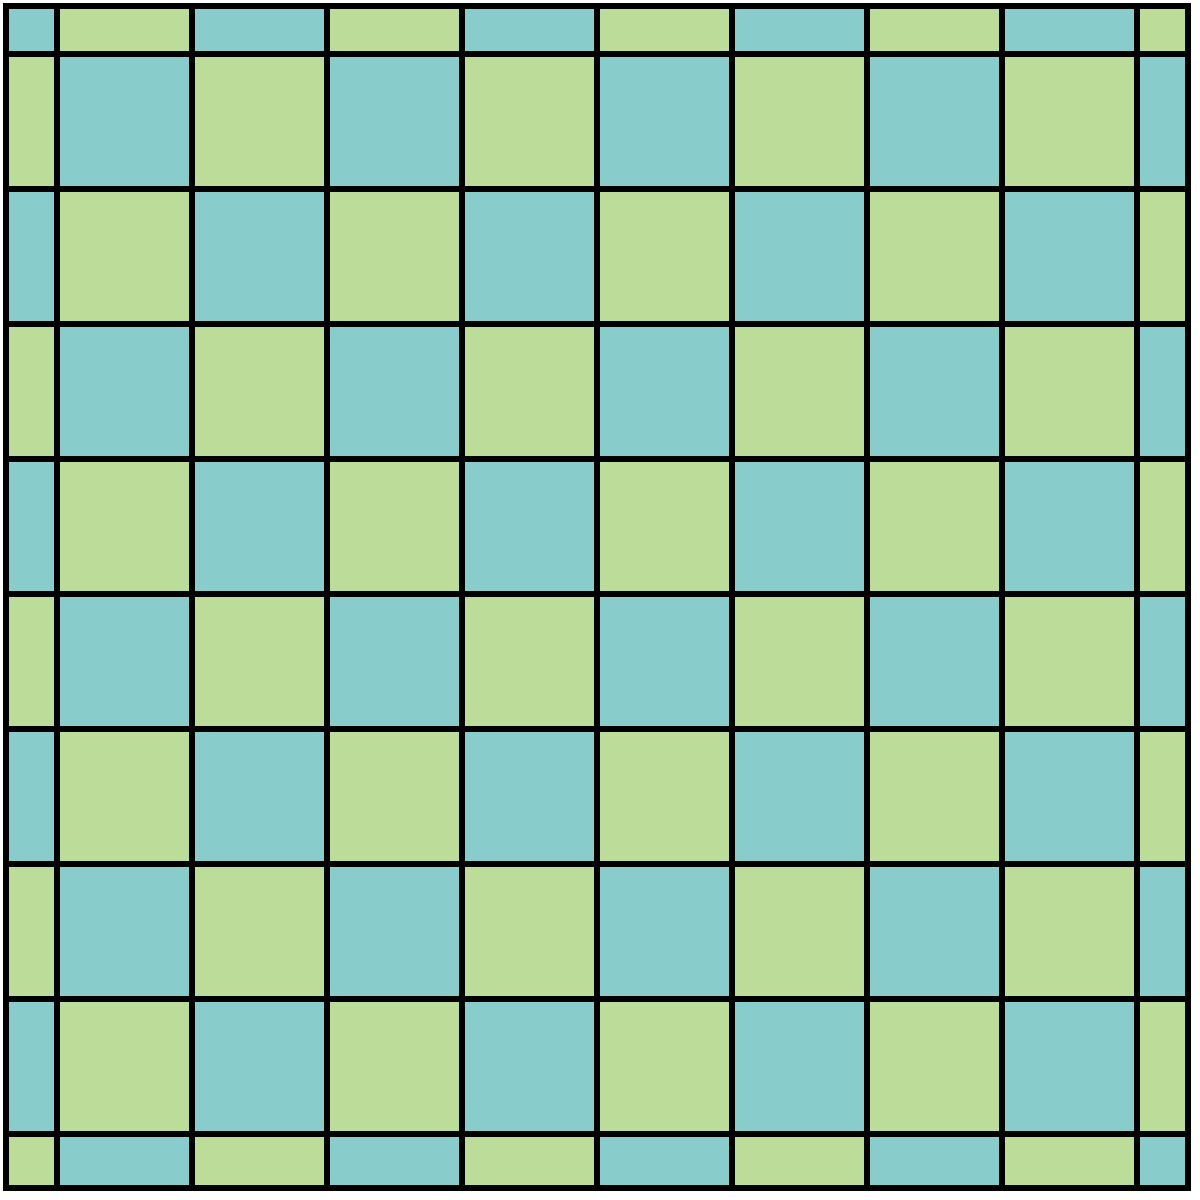
\includegraphics[width=\textwidth]{pavage_carre.png}
                \caption{Pavage carré}
                \label{fig:pavage_carre}
            \end{subfigure}
            \quad 
            \begin{subfigure}{0.3\textwidth}
                \centering
                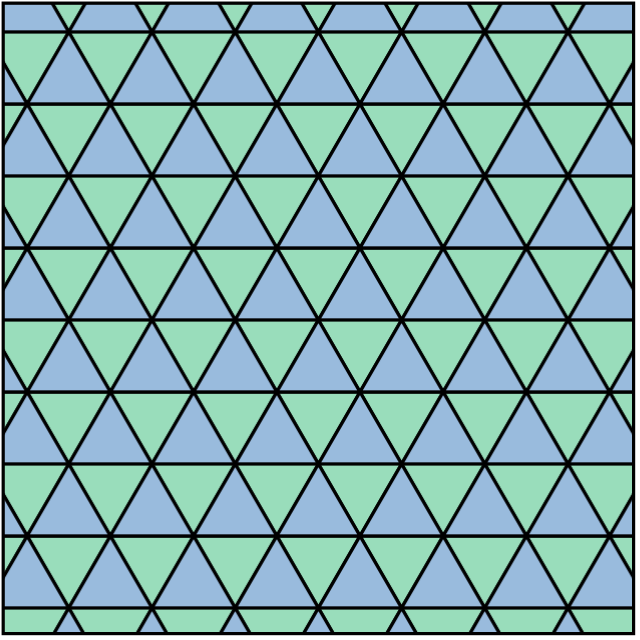
\includegraphics[width=\textwidth]{pavage_triangulaire.png}
                \caption{Pavage triangulaire}
                \label{fig:pavage_triangulaire}
            \end{subfigure}
            \caption{Les différents pavages disponibles.}
            \label{label_de_la_figure 1}
        \end{figure}
        
        
\section{Pièces et joueurs}
    \subsection{Pièces}\label{part:pawns}
        Premièrement, nous avons choisis d'implémenter de simple pions, pouvant se déplacer d'une seul case (seulement si celle-ci est vide), pour des raisons de facilité principalement. Par la suite, nous avons incorporés au jeu de nouvelles pieces, le rendant plus interessant. Chaque pièce à un déplacement particulier. \\ 
        C'est pour cela que nous avons créé une structure qui rend les pieces modulables. Chaque piece appartenant à cette structure est définit par un certain nombre d'arguments.

        \begin{lstlisting}
/** A struct representing a piece */
struct pawns_t {
    int player_index;       // Numéro du joueur propriétaire du pion
    int max_dep;            // Nombres maximum de déplacements du pion
    enum color_t color;     // Couleur du pion
    enum sort_t type;       // Type du pion
    int position;           // Position du pion
    int captured;           // Etat du pion
};\end{lstlisting}

        \noindent Nous avons implémenté plusieurs types de pions : \\
            
        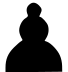
\includegraphics[width=0.45cm]{pawn.png} \textbf{Le Pion simpe :} \\
        Le pion est la pièce basique du jeu, il possède un seul mouvement dans la direction de son choix. Cependant il est possible d'en faire une dame d'echec en augmentant simplement son nombre de mouvement maximum afin qu'il puisse se déplacer sur de plus grandes distances.\\
            
        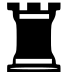
\includegraphics[width=0.45cm]{tower.png} \textbf{La Tour :} \\
        Elle peut, comme aux échecs, se déplacer seulement en direction des points cardinaux. Nous avons décidé de limiter ses déplacement au Max(longueur du plateau, largeur du plateau). En effet, sans cette condition, étant donné l'apparence torique de notre plateau, ses movements pourrait être infinis. \\
            
        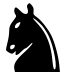
\includegraphics[width=0.45cm]{elefun.png} \textbf{L'éléphant :} \\
        Il se déplace uniquement suivant les 4 directions cardinales, dans le cas de base, il dispose de deux déplacement succésifs, mais cette valeur peux être modifiée. \\
            
        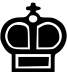
\includegraphics[width=0.45cm]{king.png} \textbf{Le Roi premier :} \\
        Il se téléporte directement sur une case portant un numéro premier, si celle-ci n'est pas occupé par un autre pion. \\
    
    \subsection{Joueurs}
        Un minimum de deux joueurs est nécessaire pour lancer une partie. Chaque joueur est associé à un index unique. Ils possèdent aussi une couleur, un nombre de pièces ainsi qu'un tableau qui les contients. La structure se présente comme ceci :
        \begin{lstlisting}
/** A struct representing a player */
struct players_t {
    int index;                          // Numéro du joueur 
    int pawns_nb;                       // Nombre de pièces
    struct pawns_t pawns[WORLD_SIZE/2]; // Tableau des pièces du joueur 
    enum color_t color;                 // Couleur du joueur
};\end{lstlisting}

    Le jeu peut également être joué à plus de deux joueurs en fonction de la taille du monde. L'implémentation de joueur tient à respecter l'équilibre du jeu. Donc si le plateau ne permet pas de répartir un certain nombre de joueurs différents à l'initialisation alors cet équilibre est romput. 
    \subsection{Formations de départ}
            Pour plus de diversité, nous avons mis en place deux formations de départs différentes. Une premiere, classique, resemblant aux echecs (mais toujours en prennant en considération la forme torique de notre plateau). \\
            
            \begin{figure}[H]
                \centering
                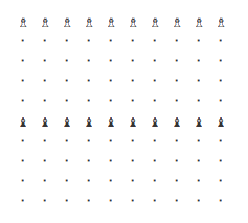
\includegraphics[scale=0.6]{departclassique.png}
                \caption{Départ classique}
                \label{fig:depart_classique}
            \end{figure}

            La deuxième formation que nous avons implémentée est plus particulière et présente le plateau sous forme de champs de bataille, avec des énorme blocs de pièces séparés par des tranchés. Cette formation avait à l'origine pour but de tester la réaction des pièces lorsqu'elles sont entourées de plein d'autres. \\
            
            \begin{figure}[H]
                \centering
                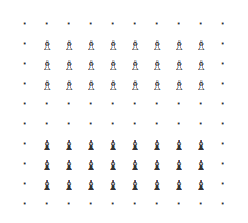
\includegraphics[scale=0.6]{img/battleground.png}
                \caption{Départ champ de bataille}
                \label{fig:depart_champ_de_bataille}
            \end{figure}

            Le type de pions qui composent ces formations est modulable. Par défaut, la formation est remplie avec des pions simples. Néanmoins il est possible de changer cette pièce par défaut, ou encore d'ajouter un certain nombre de pièces "spéciales" en plus de la pièce par défaut. La position de ces pièces est choisie par le programme. Pour celà nous avons implémenté un algorithme qui, en fonction du nombre de pièces spéciales à placer, choisis une formation qui soit identique pour chaque joueur et qui ne crée pas de déséquilibre entre les joueurs, et ceci quelque soit le nombre de joueur. \\
            La figure \textbf{\ref{fig:depart_classique_a_4}} montre les positions de départ pour une partie lancée avec 4 joueurs, sur un monde de taille $10\times10$, avec  $2$ tours (pièce) par joueurs.
            
            \begin{figure}[H]
                \centering
                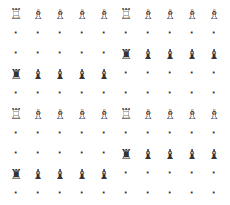
\includegraphics[scale=0.6]{img/depart_classique_a_4.png}
                \caption{Départ classique à 4}
                \label{fig:depart_classique_a_4}
            \end{figure}
            
    \section{Boucle de jeu}

        \subsection{Sélection des options}
            Toujours dans le but d'augmenter la modularité de notre jeu, nous avons rendu un maximum d'options au choix de joueur lors du l'exécution. Les choix se font par l'intermédiaire de paramètres à ajouter lors de l'exécution du programme. Si les options sont écrites de manières incorrectes, le programme ne les prendra pas en compte et utilisera des valeurs par défaut.
            
        \subsection{Déroulement d'une partie}
            Lorsque le programme est lancé, le programme initalise un "monde extérieur", que nous verons plus tard et qui contient le plateau de jeu, les joueurs et leur pièces. \\
            \newline
            Au début de chaque tour un controle sur le changement de térrain est effectué afin de le modifié si il est nécéssaire d'après les options de l'utilisateur. \\
            Ensuite une pièce du joueur est choisit au hasard pour se déplace dans l'une des cases accessible aléatoirement. Puis on vérifie si il y a un vainquer  ou si le max de tours à été atteint. Dans ce cas précis le jeu s'arrete et l'indique à l'utilisateur sinon on passe au tour suivant.
            
        \subsection{Conditions de victoire}
            Notre jeu admet deux conditions de victoire différente :\\
            \begin{itemize}
                \item La première signe la fin du jeu dès lors qu'une piece arrive dans les positions de départs de l'adversaire. Cette condition est 'simple' afin de véifier les déplacements de nos pieces et le bon fonctionnement du jeu.\\
                \item La seconde elle nécésite que la totalité des pieces arrivent dans les positions de départ de ou des adversaires. Celle-ci est beaucoup plus complèxe et nécéssite des déplacements guidé pour l'atteindre. Cependant elle permet de faire durer plus longtemps les arties notament en mode 'Champ de bataille' afin de voir beaucoup d'intéractions.
            \end{itemize}